\chapter{Architecture}
\label{ch:architecture}

\begin{quotation}
“The greatest pleasure in life is doing what people say you cannot do.”
{\small\it -- Walter Bagehot (British political Analyst, Economist and Editor, one of the most influential journalists of the mid-Victorian period.1826-1877) }
\end{quotation}

This chapter explains the design goals, main architecture, and the protocols we present as solution to the problem of distributed data stores regarding consistency versus availability, also introduced in earlier chapters. Rather than just considering a fixed consistency model, we aim at providing finer-grained levels of consistency during data replication, and taking as an example social networks such as Facebook~\footnote{http://www.facebook.com}, we showcase how one might not need so strict consistency depending on what updates are replicated. For that, will be explored how bounded data semantics help to achieve that goal.

First of all, we take a general overview of the system design in Section~\ref{architecture:overview}. Following sections in the chapter reflect the architecture of the system in terms of network as well software components. Each of the steps in the design process has been carefully justified in order to integrate well in the original system architecture, and in particular those decisions related to asynchronous replication using Remote Procedure Call~\footnote{RPC, http://en.wikipedia.org/wiki/Remote\_procedure\_call} mechanisms that are the base of the architectural changes introduced with a custom HBase-QoD module.


%% **** TODO STOP *** rewrite chapter overview

In order to achieve that, it is necessary to take into account a set of requirements that help at addressing the challenges and fulfilling our goals, that are described  in Section~\ref{architecture:requirements}. Section~\ref{architecture:network} presents the network architecture where HBase-Qod operates. In Section~\ref{architecture:consistency}, we describe the consistency model proposed for HBase-QoD, including operation grouping, and its enforcement. The chapter closes with the software architecture of the extensions proposed to HBase.


  %%%%%%%%%%%%%%%%%%%%%%%%%%%%%%%%%%%%%%%%%%%%%%%%%%%%%%%%%%%%%%%%%%%%%%%%%%%%%
  %
%%%%%                        SECTION
 %%%
  %

% How the containers replicate thigns with the QoD
%reprise overall system overview of HBase (if needed check approach in papers such as BigTable or HBase papers/docs) kind of usage overview, applications, storage, data centers, etc. (the 1000 feet view or birds-eye view)



\section{System Architecture Overview}\label{architecture:overview}
%%%% TODO STOP REWRITE THIS TEXT FOLLOWING THE NEW STRUCTURE OF THE CHAPTER
We start by showing the logic behind the main architectural design decisions and showcase scenarios as in a "thousand feet view" of the system, which provides an overview of the system first of all such as in Figure~\ref{fig-high-level}. Following, we delve into the proposed changes in order to verify the feasibility of the implementation as well as what scenarios are best suited to our definition of consistency.

%insert 1000 feet view
\begin{figure}[h]
\centering
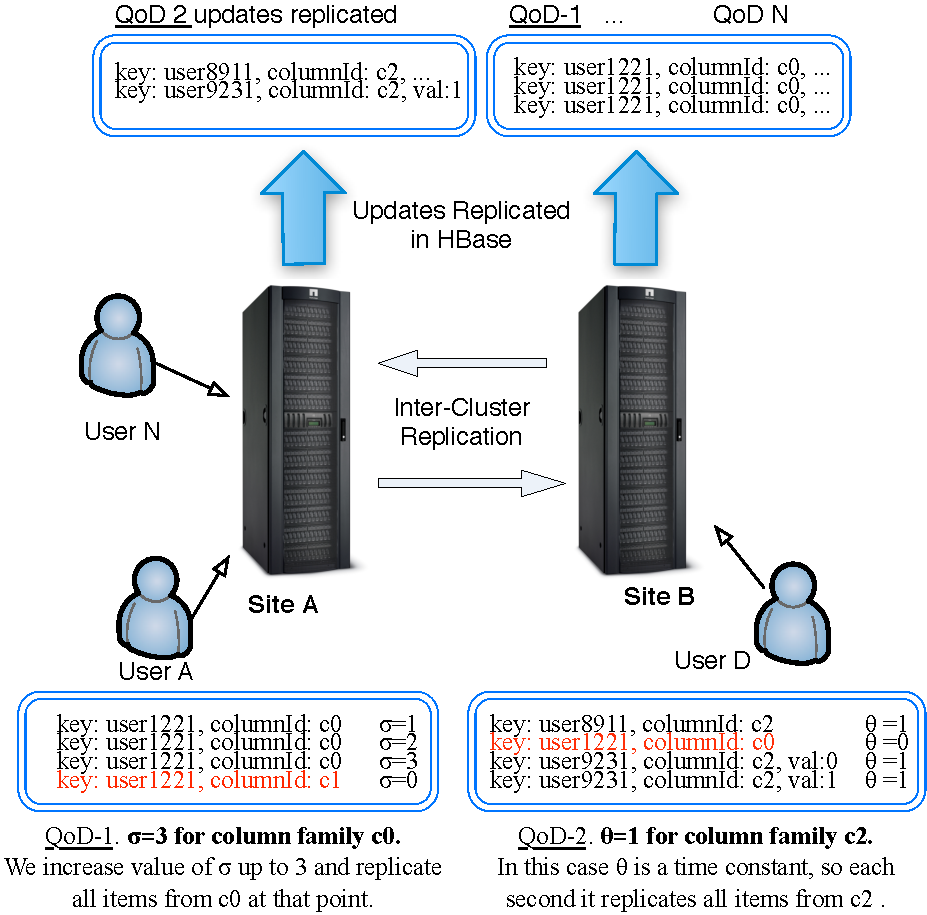
\includegraphics[width=0.8\linewidth]{figs/highlevel.pdf}
\caption{HBase QoD high-level}
\label{fig-high-level}
\end{figure}


In order to introduce a new HBase-QoD module architecture, the first step is to study in details the existing system to get familiar with it and identify the best locations for new code added. Therefore, taking into account the original architecture inner-workings of the data store at the logical level will ensure correctness and validity of the new architecture here presented as well as prototype described in next chapter.

\begin{enumerate}
\item First identifying the source and destination of updates.
\item Secondly, defining a QoD vector-model based on the schema design of HBase so we can reach our goals.
\item Finally integrating both parts into the same system, and providing a mechanism to switch on and off the module at run time into HBase.
\end{enumerate}

% Implementation details, such as WALEdit, algorithm, images of QoD inside DC, etc.
HBase is written in Java and its replication mechanisms are related to a Write Ahead Log (WAL) that also ensures durability of updates and disaster recovery. Replication must be enabled for shipping updates between peer cluster locations in remote or nearby data centers. The process of replication is carried out asynchronously so there is not additional overhead or latency introduced in the the master server during that operation.  Although, since the process is not strongly consistent, in write heavy applications a slave can have stale data in the order of more than just a few seconds according to the eventual consistency approach.

Therefore, until the last update first commits to the local disk, it cannot be seen replicated in a remote location. To keep control of staleness, we plug a QoD module called HBase-QoD which provides and takes advantage of a filtered and sorted by priority queue of items later scheduled for replication accordingly. Thereafter, when the method completes, updates are shipped in an ordered fashion by defining and enforcing bounds on data as key decision properties for their delivery to a remote cluster location. For write intensive applications that can be both beneficial in terms of peaks of bandwidth usage and also reduced staleness of data.

Given that HBase provides eventual consistency mechanisms through Remote Procedure Calls in order to replicate items, that data store is chosen as system use case to firstly introduce the proposed architecture here. Also, we can enhance the current multi-row atomic model, using an approach that can also relate column families between updates in order to provide the same atomicity at the column-level.

%\paragraph*{Data Center Storage View:}
The physical structure of column families is outlined in Table~\ref{tab:hbase-model}, where we have a view of its data model. That is potentially useful for distinguishing updates between cluster update owners and users or applications that need those updates from another cluster for the fact of being consistently up to date in regards to their own local data center ongoing update operations.

%The overall architecture layout is presented in Figure~\ref{fig-high-level}. The module that introduces the vector-field consistency model is shown in Algorithm~\ref{algo1}, and follows the architectural design choices of HBase as well as the main goals here desired. In addition to that, in Section~\ref{grouping} we also explain how to group updates and what are the benefits of doing that.

%\paragraph*{Replication Flow:}
Replication occurs in two different manners into HBase. Intra-cluster and Inter-Cluster. We target the later, so firstly, we set up a standalone Zookeeper~\footnote{http://zookeeper.apache.org/} on each server running, and therefore separate clusters with a master server each. This is useful for enabling and testing HBase-QoD performance.

Secondly, a cluster with a distributed Zookeeper ensemble on each of the nodes is configured, and we will aim to also test intra-cluster scenarios for HBase-QoD even though that is not our main goal. This benchmark use case can be also useful to us for testing weak consistency features presented into YCSB++\footnote{http://www.pdl.cmu.edu/ycsb++/}.

%\paragraph*{Usage}
%The usage of HBase-QoD is straight-forward and integrated into HBase core architecture. % keep writing here about cli possible function (ruby)
%The configuration for that is shown in the following Figure~\cite{}

\begin{center}
\begin{table}\label{tab:hbase-model}
\centering
\begin{tabular}{ |l|l|l|l| }
\hline
Row Key & Timestamp & Column & Value \\ \hline
\multirow{3}{*}{com.gsd.inesc-id.www} & T1 & anchor:inesc-id.gsd.com & value1\\
 & T1 & anchor:domain2.com & value2\\
 & T2 & anchor:domain3.com & value3\\
 \hline
\end{tabular}
\caption{This table shows the physical structure of HBase data model}
\end{table}
\end{center}



%%%%%%%%%%%%%%%%%%%%%%%%%%%%%%%%%%%%%%%%%%%%%%%%%%%%%%%%%%%%%%%

\section{From eventual consistency to QoD consistency}\label{architecture:requirements}
This section explains the motivation of the steps taken in regards to the design decisions adopted in order to present an enhanced architecture that also follows best practices in regards to code readability and re-usability for the system of choice. In the following sections of the chapter we justify the 'how' and 'why' of the choices we have made during the development process later once we have a well-rounded architecture of the intended replication module for HBase.

With eventual consistency enforcement in place, updates and insertions are propagated asynchronously between clusters so Zookeeper is used on each of them for storing their positions in log files that hold pointers to the next log entry to be shipped when replicated from/to other HBase cluster. To ensure cyclic replication (master to master) and prevent from copying same data back to the source, a sink location with remote procedure calls invoked is already into place with HBase, so we use the current features provided by HBase in that regard. Therefore if we can control the edits to be shipped, we can also decide what is replicated, when or in other words, how soon or often.

Design Goals are as follows:

\begin{enumerate}
\item Separation of concerns between replication data semantics. Applied to HBase can provide different levels of consistency among updates.
\item Replication can be still asynchronous but with higher degree of consistency guarantees, based on a vector-field consistency model that allows defining constraints and limits applied to updates that have as target different client application data.
\item Partitioning allowed with eventual consistency allowing to reconcile changes autonomously, while grouping of operations enforces maintaining atomically replicated updates so avoiding the first in case of long periods of disconnection to the network (it is already possible to define a retry timeout in HBase in case of partitioning so we do not need to focus on that but rather on the grouping part)
\end{enumerate}

\subsection{Challenges addressed in HBase-QoD}

How long does it take for edits to be propagated to a slave cluster? This is one of the main questions that can strike Cloud Architects when it comes to distributed NoSQL architectures. As noted in the HBase forums, there is a increasing interest in knowing how and when data is propagated to slave clusters. For instance to separate clients facing HBase clusters and the ones used to to run benchmarks and analysis that involves heavy Map Reduce tasks that are very scan intensive.

\paragraph*{Buffering in HBase:}
As noted by Jean-Daniel Cryans, replication acts as soon as the buffer itself is full or it reaches the end of the file (EOF). The end of a file is determined by when a file is reopened because there is no way to tail a file into HDFS without closing a previous reader, therefore reopening the file and seeking to a certain position it is required. As a consequence, replication is not able to keep filling the buffer for minutes before sending because it quickly gets to the end of the file anyway. The HBase replication stream is almost always in the range of sub-seconds lag. Only if it reaches the end of a file and it does not read anything new, then that will be waiting for new updates to arrive.

In the case of \emph{ReplicationSource}, that tails the WAL and sends the WALEdit to the ReplicationSink via RPC. In other words, the code applies the edits to the slave cluster via a remote call to the method in the RPC sink (calling a method named \emph{ReplicateLogEntries} remotely).

In order to control that, HBase-QoD modifies the internals of buffering WALs at the source that will be sent to a sink location.

\paragraph*{Configurations:}
There is a set of configurations in HBase to control how updates are replicated. That is contained in XML file called hbase-site.xml.

\begin{enumerate}
\item replication.source.size.capacity, default is 64MB but recently so that is possibly too big.
\item replication.source.nb.capacity, default is 25k. The buffer is flushed when either size or capacity is reached but what really important is the size.
\item replication.source.maxretriesmultiplier, default is 10, so it retries up to 10 times with pauses that are currentIteration times.
\item replication.source.sleepforretries. By default it sleeps 1 sec, 2, 3, 4... 9, 10, 10, 10, 10 until it's able to replicate (default is 1)
\end{enumerate}

Although useful, currently those mechanisms do not allow differentiation between data priority when it comes to flushing updates to slave cluster. Therein HBase-QoD described next is devised to see how it can help in that regard.


%%%%%%%%%%%%%%%%%%%%%%




  %%%%%%%%%%%%%%%%%%%%%%%%%%%%%%%%%%%%%%%%%%%%%%%%%%%%%%%%%%%%%%%%%%%%%%%%%%%%%
  %
%%%%%                        SECTION
 %%%
  %

\section{Network Architecture and Protocols}\label{architecture:network}
% - diagrams and clear explanations of how HBase and its distribution and replication works within data center and across data centers this is where your diagrams should show up describing the information flows and where QoD is to be applied.
At the Replication Level, the network architecture is as shown in Figure ~\ref{fig-replication-level}. Which reflects the main components at each site by exposing them into adjacent layers which interact with each other. The flow is both, upwards and downwards the stack in each of the Master servers of HBase in the distributed cluster set up at INESC-ID.

\begin{figure}[t]
\centering
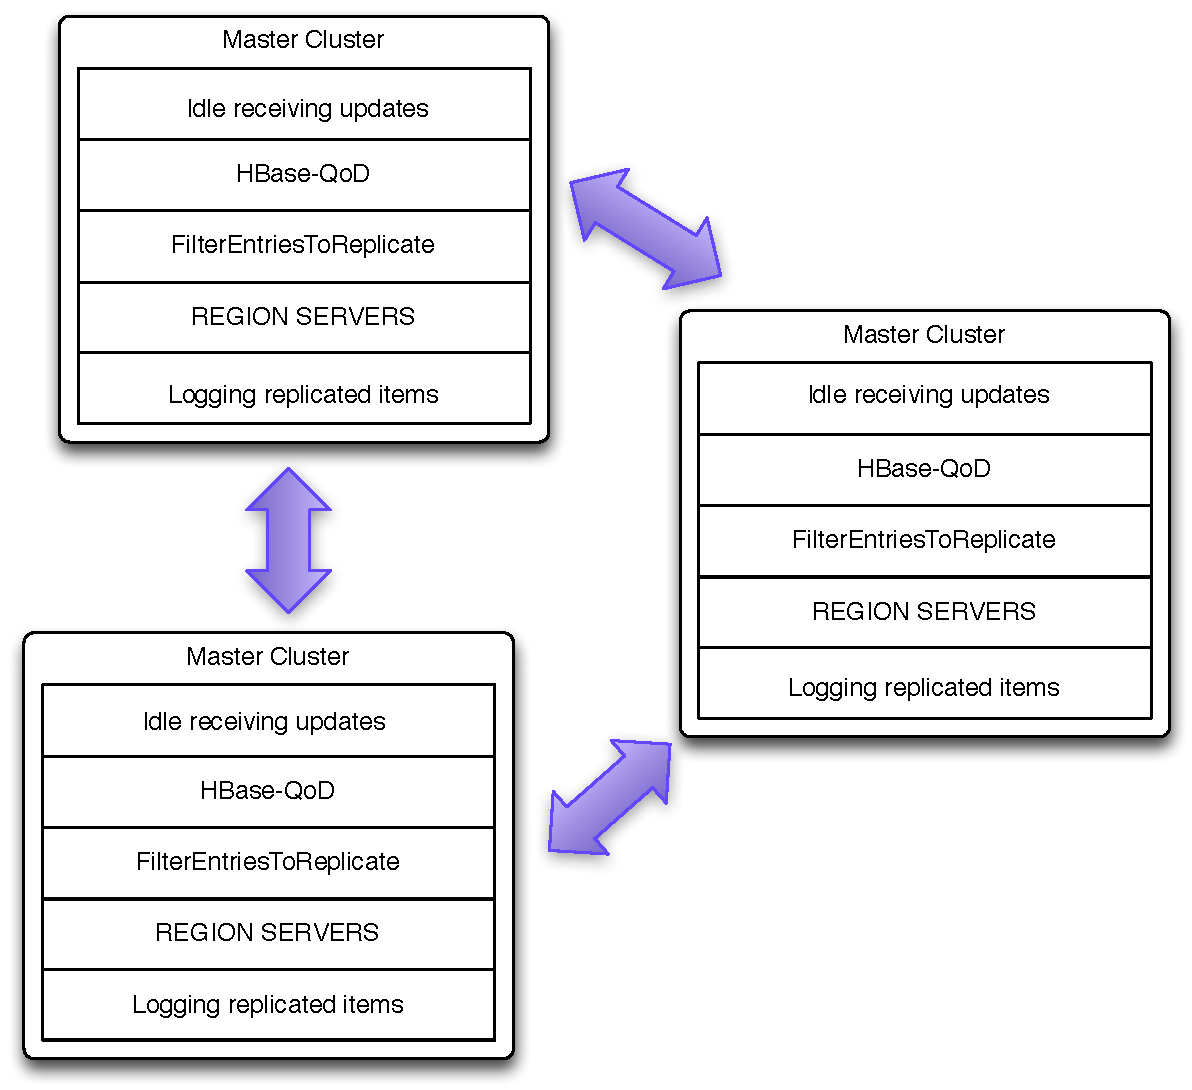
\includegraphics[width=0.8\linewidth]{figs/ReplicationFlow.pdf}
\caption{Replication Flow of updates}
\label{fig-replication-level}
\end{figure}

%\paragraph*{*****Prototypical Example}
% complete example of usage, that I think you are presenting in the implementation. describe how a client application program  can specifiy the Qod and operationg groupings so that the reader sees everything now in a complete example (this may be shown earlier but I think it is a good way of wrapping up everything and make it more clear)
We extend HBase, adding updates due to be replicated in a priority queue according to their own QoD in each case. Thereafter once the specified QoD threshold is reached another thread from HBase in the form of Remote Procedure Call collects and ships all of them at once.

\begin{figure}[t]
\centering
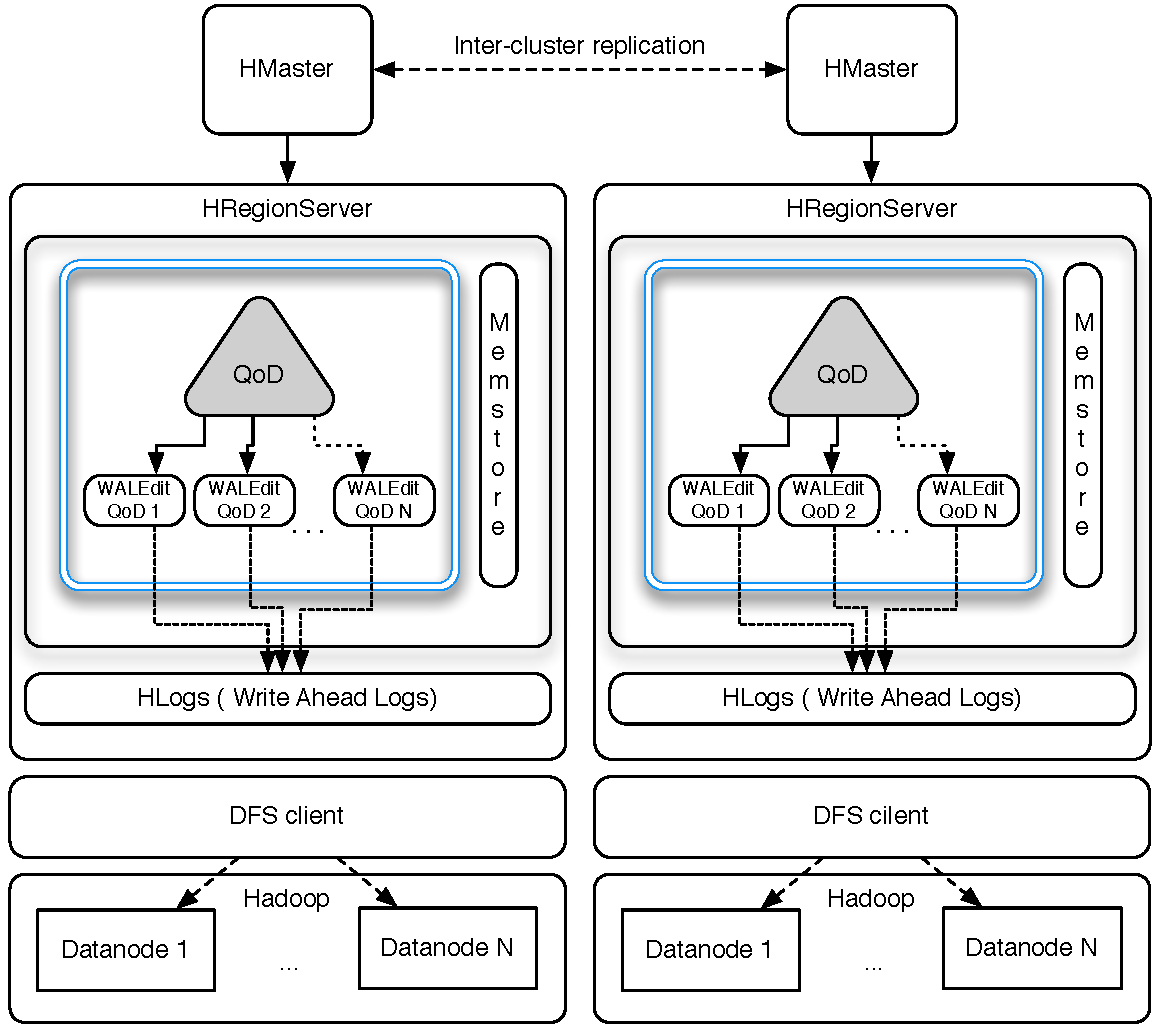
\includegraphics[width=0.8\linewidth]{figs/multi-site.pdf}
\caption{HBase QoD operation}
\label{fig-qod-module}
\end{figure}

In Figure~\ref{fig-qod-module} we observe the QoD module plugging into HBase, intercepting the incoming updates from the upper layers and passing them down and the resulting outcome to the Write Ahead Logs for later replication.

%\paragraph*{Remote Procedure Calls}
HBase implements remote procedure calls for the replication of items between servers or clusters. These mechanisms have been proven a useful paradigm for providing communication across computer networks for several reasons~\cite{Birrell:1984}. An RPC mechanism is mainly responsible for providing control of data transfers between a source and a destination location. In the case of HBase, these are called \emph{ReplicationSource.java} and \emph{ReplicationSink.java} respectively. To understand in depth that topic, it has been discussed in as much depth as possible with Apache Foundation contributors for the HBase community. That is helpful to clarify and understand better how the system operates before introducing the changes proposed with our HBase-QoD.



%\section{System Architecture}
% architecture inside each HBase instance with your new modules.
%A three-dimensional vector constraint model based on~\cite{Santos:2010} is implemented in the form of the corresponding QoD paradigm, shipping updates for replication, or retaining them for later shipment as mentioned. For that to be possible, we have used a set of customized data structures, which hold the values of the database rows we desire to check according to some specific field we might be interested in (e.g column family) for replication.

\section{QoD Consistency Enforcement}\label{architecture:consistency}
% description of the VFC algorithms and how the consistency is enforced whan updates arrive , etc. this also includes operation grouping (only code like details should be left for the implamentations, e.g., the listings that you show there and are ok).
%% Start by presenting our model, constraints, data containers, and how things work (are enforced / evaluated )

Consistency enforcement in HBase-QoD is inspired in three-dimensional vector constraint model based on~\cite{Santos:2010}, and adapted to HBase in order to drive shipping updates for replication, or retaining them for later shipment as mentioned. For that to be possible, we have used a set of customized data structures, which hold the values of the database rows we desire to check according to some specific field we might be interested in (e.g column family) for replication.

The QoD paradigm implemented allows for entries to be evaluated prior to replication based on one or several of the three parameters in a three-dimensional vector K ($\theta$, $\sigma$, $\nu$), corresponding to Time, Sequence, Value respectively in our case. Secondly, we take care of updates that collide with previous ones (same keys but different values). They can also be checked for number of pending updates or value difference from previously replicated updates, and then shipped or kept on the data structure accordingly. The time constraint can be always validated every X seconds, and the other two constraints are validated through Algorithm.~\ref{algo1}, whenever updates arrive. For the work presented here we use Sequence ($\sigma$) as the main vector-field bound (\texttt{HBaseQoD.enforce(containerId)}).

% architecture inside each HBase instance with your new modules.
The original HBase architecture has built-in properties derived from the underlying HDFS layer. As part of it, the WALEdit data structure is used to store data temporarily before being replicated, useful to copy data between several HBase locations. The QoD algorithm (shown in Algorithm.~\ref{algo1}) uses that data structure, although we extend it to contain more meaningful information that help us in the management of the outgoing updates marked for replication.

% High-level algorithm we use to modify queued items for replication
\begin{algorithm*}
\caption{QoD high-level algorithm for filtering updates}
\label{algo1}
\begin{algorithmic}[1]
\REQUIRE $containerId$
\ENSURE $maxBound \neq 0$ and $controlBound \neq 0$
%\STATE $y \leftarrow 1$
\WHILE{$enforceQoD (containerId)$}
\IF{$getMaxK(containerId) = 0$}
\RETURN $true$
\ELSE[$getactualK(containerId)$]
\STATE $actualK(\sigma) \leftarrow actualK(\sigma)+1$
	\IF{$actualK(\sigma) \geq containerMaxK(\sigma)$}
	\STATE $actualK(\sigma) \leftarrow 0$
	\RETURN $true$
	\ELSE
	\RETURN $false$
	\ENDIF
\ENDIF
\ENDWHILE
\end{algorithmic}
\end{algorithm*}

To compare and track the QoD fields, that act as constraints to replicate updates, against these stored entries, we defined data \emph{containers} which are useful to keep track of the current value of the vector-field selected to bound replication to, and secondly the maximum value it will be allowed to reach before updates are flushed to the slave cluster and then reset again. That is as what we call the QoD percentage of updates replicated (according to the selected vector-field bound, e.g $\sigma$). The process is partly automated, of by now, we just define it at run-time (or by the developer later) by adding a parameter into the system console to define a vector-field specific bound.

\subsection{Caching updates}\label{architecture:caching}
The problem with controlling the flow of updates for shipping through replication is indeed what to do with them until one is able to handle them appropriately. Therefore it is devised a \emph{Unified Caching} layer into HBase-QoD, which serves as a helper to keep track of items and their priority for replication. When an update is received and the QoD bound is reached, the Cache is either emptied and updates are shipped or it is starting to be filled again. That allows to differentiate between \textbf{Critical} and \textbf{Non-Critical} updates.

\subsection{Operation Grouping}\label{grouping}
At the application level, it may be useful for HBase clients to enforce the same consistency level on groups of operations despite affected data containers having different QoD bounds associated. In other words, there may be specific situations where write operations need to be grouped so that they can be all handled at the same consistency level and propagated atomically to slave clusters. 

For example, publication of user statuses in social networks is usually handled at eventual consistency, but if they refer to new friends being added (e.g., an update to the data container holding the friends of a user), they should they should be handled at a stronger consistency level to ensure they are atomically visible along with the list of friends of the user in respect to the semantics we describe here.

In order to not violate QoD bounds and maintain consistency guarantees, all data containers of operations being grouped must be propagated either immediately after the block execution, or when any of the QoD bounds associated to the operations has been reached. When a block is triggered for replication, all respective QoD bounds are naturally reset. 

To enable this behavior we propose extending the HBase client libraries to provide atomically consistent blocks.
Namely, adding two new methods to HTable class in order to delimit the consistency blocks: \textit{startConsistentBlock} and \textit{endConsistentBlock}. Each block, through the method \textit{startConsistentBlock}, can be parameterized with one of the two options: i) \textit{IMMEDIATE}, which enforces stronger consistency for the whole block of operations within it; and ii) \textit{ANY}, which replicates a whole block as soon as any QoD vector field bound, associated with an operation inside the block is reached.

Next, in Listing~\ref{lst:group-listing} we provide an illustrative simple example of a social network where three containers with different consistency levels are modified. Note that we are not aiming at full transactional support, as it would be possible to change the same data containers modified by a set of grouped operations, at the same time, from other operations individually.

\begin{lstlisting}[language={java}, caption={Operation grouping},label={lst:group-listing}]
htable.startConsistentBlock(ConsistencyType.IMMEDIATE)
Put put1 = new Put(Bytes.toBytes("row1"));
put1.add(Bytes.toBytes("SocialNetTable"),Bytes.toBytes("status"), Bytes.toBytes("friend 12345 added"));

Put put2 = new Put(Bytes.toBytes("row2"));
put2.add(Bytes.toBytes("SocialNetTable"), Bytes.toBytes("friends"), Bytes.toBytes("12345"));

Put put3 = new Put(Bytes.toBytes("row3"));
put3.add(Bytes.toBytes("SocialNetTable"), Bytes.toBytes("wall"), Bytes.toBytes("12345 is now a friend"));

htable.put(put1);
htable.put(put2);
htable.put(put3);

htable.endConsistentBlock();
\end{lstlisting}

\subsection{Proposed scenario}
One of the key factors for having operations grouping working together with HBase-QoD is the depicted in Figure~\ref{fig-qod-grouping}. We can see that the operations that are grouped need to communicate over the network less often to other clusters, while arriving earlier in some cases than updates shipping as if several individual operations from location Cluster A were performed. This is due to the ability of HBase-QoD to deliver demanded updates in a consistent timely-fashion rather than on a per request arrival basis, which means possibly delaying the replication process by a fraction of the amount of communication that can be saved instead using the mentioned technique.

\begin{figure}[t]
\centering
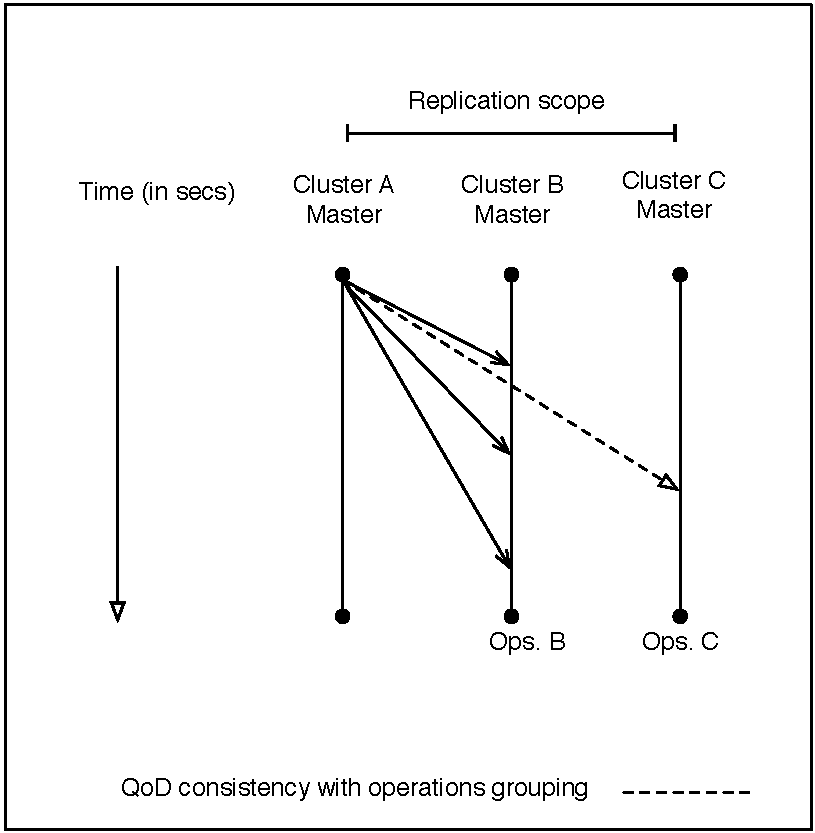
\includegraphics[scale=0.6]{figs/operation-grouping.pdf}
\caption{Resulting scenario of grouping operations in a time-lined based diagram using HBase-QoD versus a regular HBase deployment at Cluster B}
\label{fig-qod-grouping}
\end{figure}

Another experiment that has been conclusive in terms of grouping of operations is the comparison between different QoD levels, in the case of values for vector field K (-, $\sigma$, -). Setting the operation grouping for a small number of updates still shows that a timestamp in the receiving server is the same for every item in the group. The following set of operations is reflect in Figures~\ref{fig-shipping-grouping} and ~\ref{fig-receiving-grouping}. The same principle can be applied and has been demonstrated to work in the same fashion for different sets of containers.

%(table_name::columnFamily).

\begin{figure}[b]
\centering
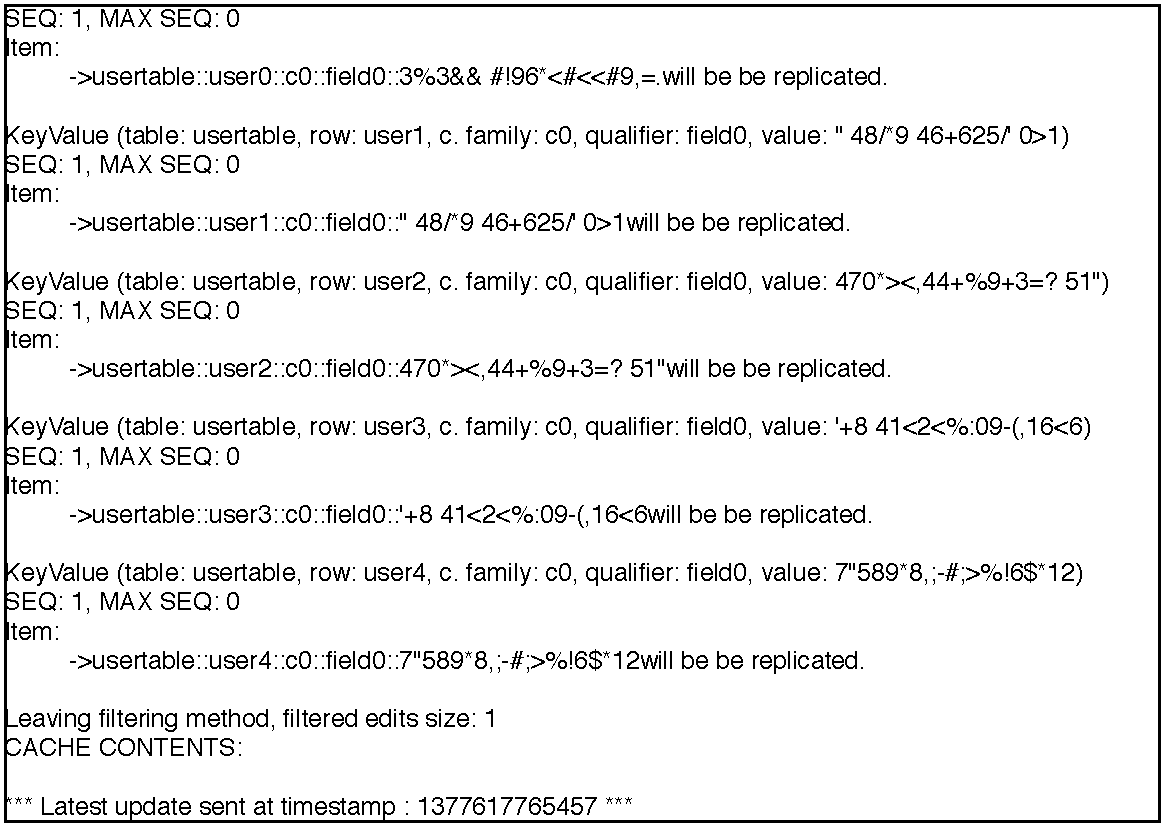
\includegraphics[scale=0.6]{figs/ginja2-grouping-send.pdf}
\caption{Sending from ginja-a2 to ginja-a1}
\label{fig-shipping-grouping}
\end{figure}

In the following Figure~\ref{fig-receiving-grouping}, we observe how the timestamp for each of the items replicated from the grouped operation have the same timestamp (\textbf{1377617765557}) at the receiving side on ginja-a1. That ensures they have arrived at the same time, and actually we verify the correctness of the experiment by leveraging internal HBase mechanisms that are currently being already used to list statistics of the age of updates sent and/or receive. At the sending side on the other hand, each update is grouped until finally they are all due to be replicated as a whole and therefore printing the timestamp only in order to comply with the reality.

\begin{figure}[t]
\centering
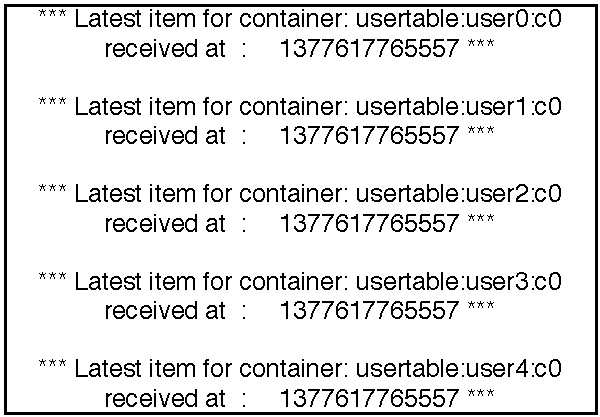
\includegraphics[scale=.6]{figs/ginja1-grouping-receive.pdf}
\caption{Receiving from ginja-a2 in ginja-a1}
\label{fig-receiving-grouping}
\end{figure}





\begin{figure}
\centering
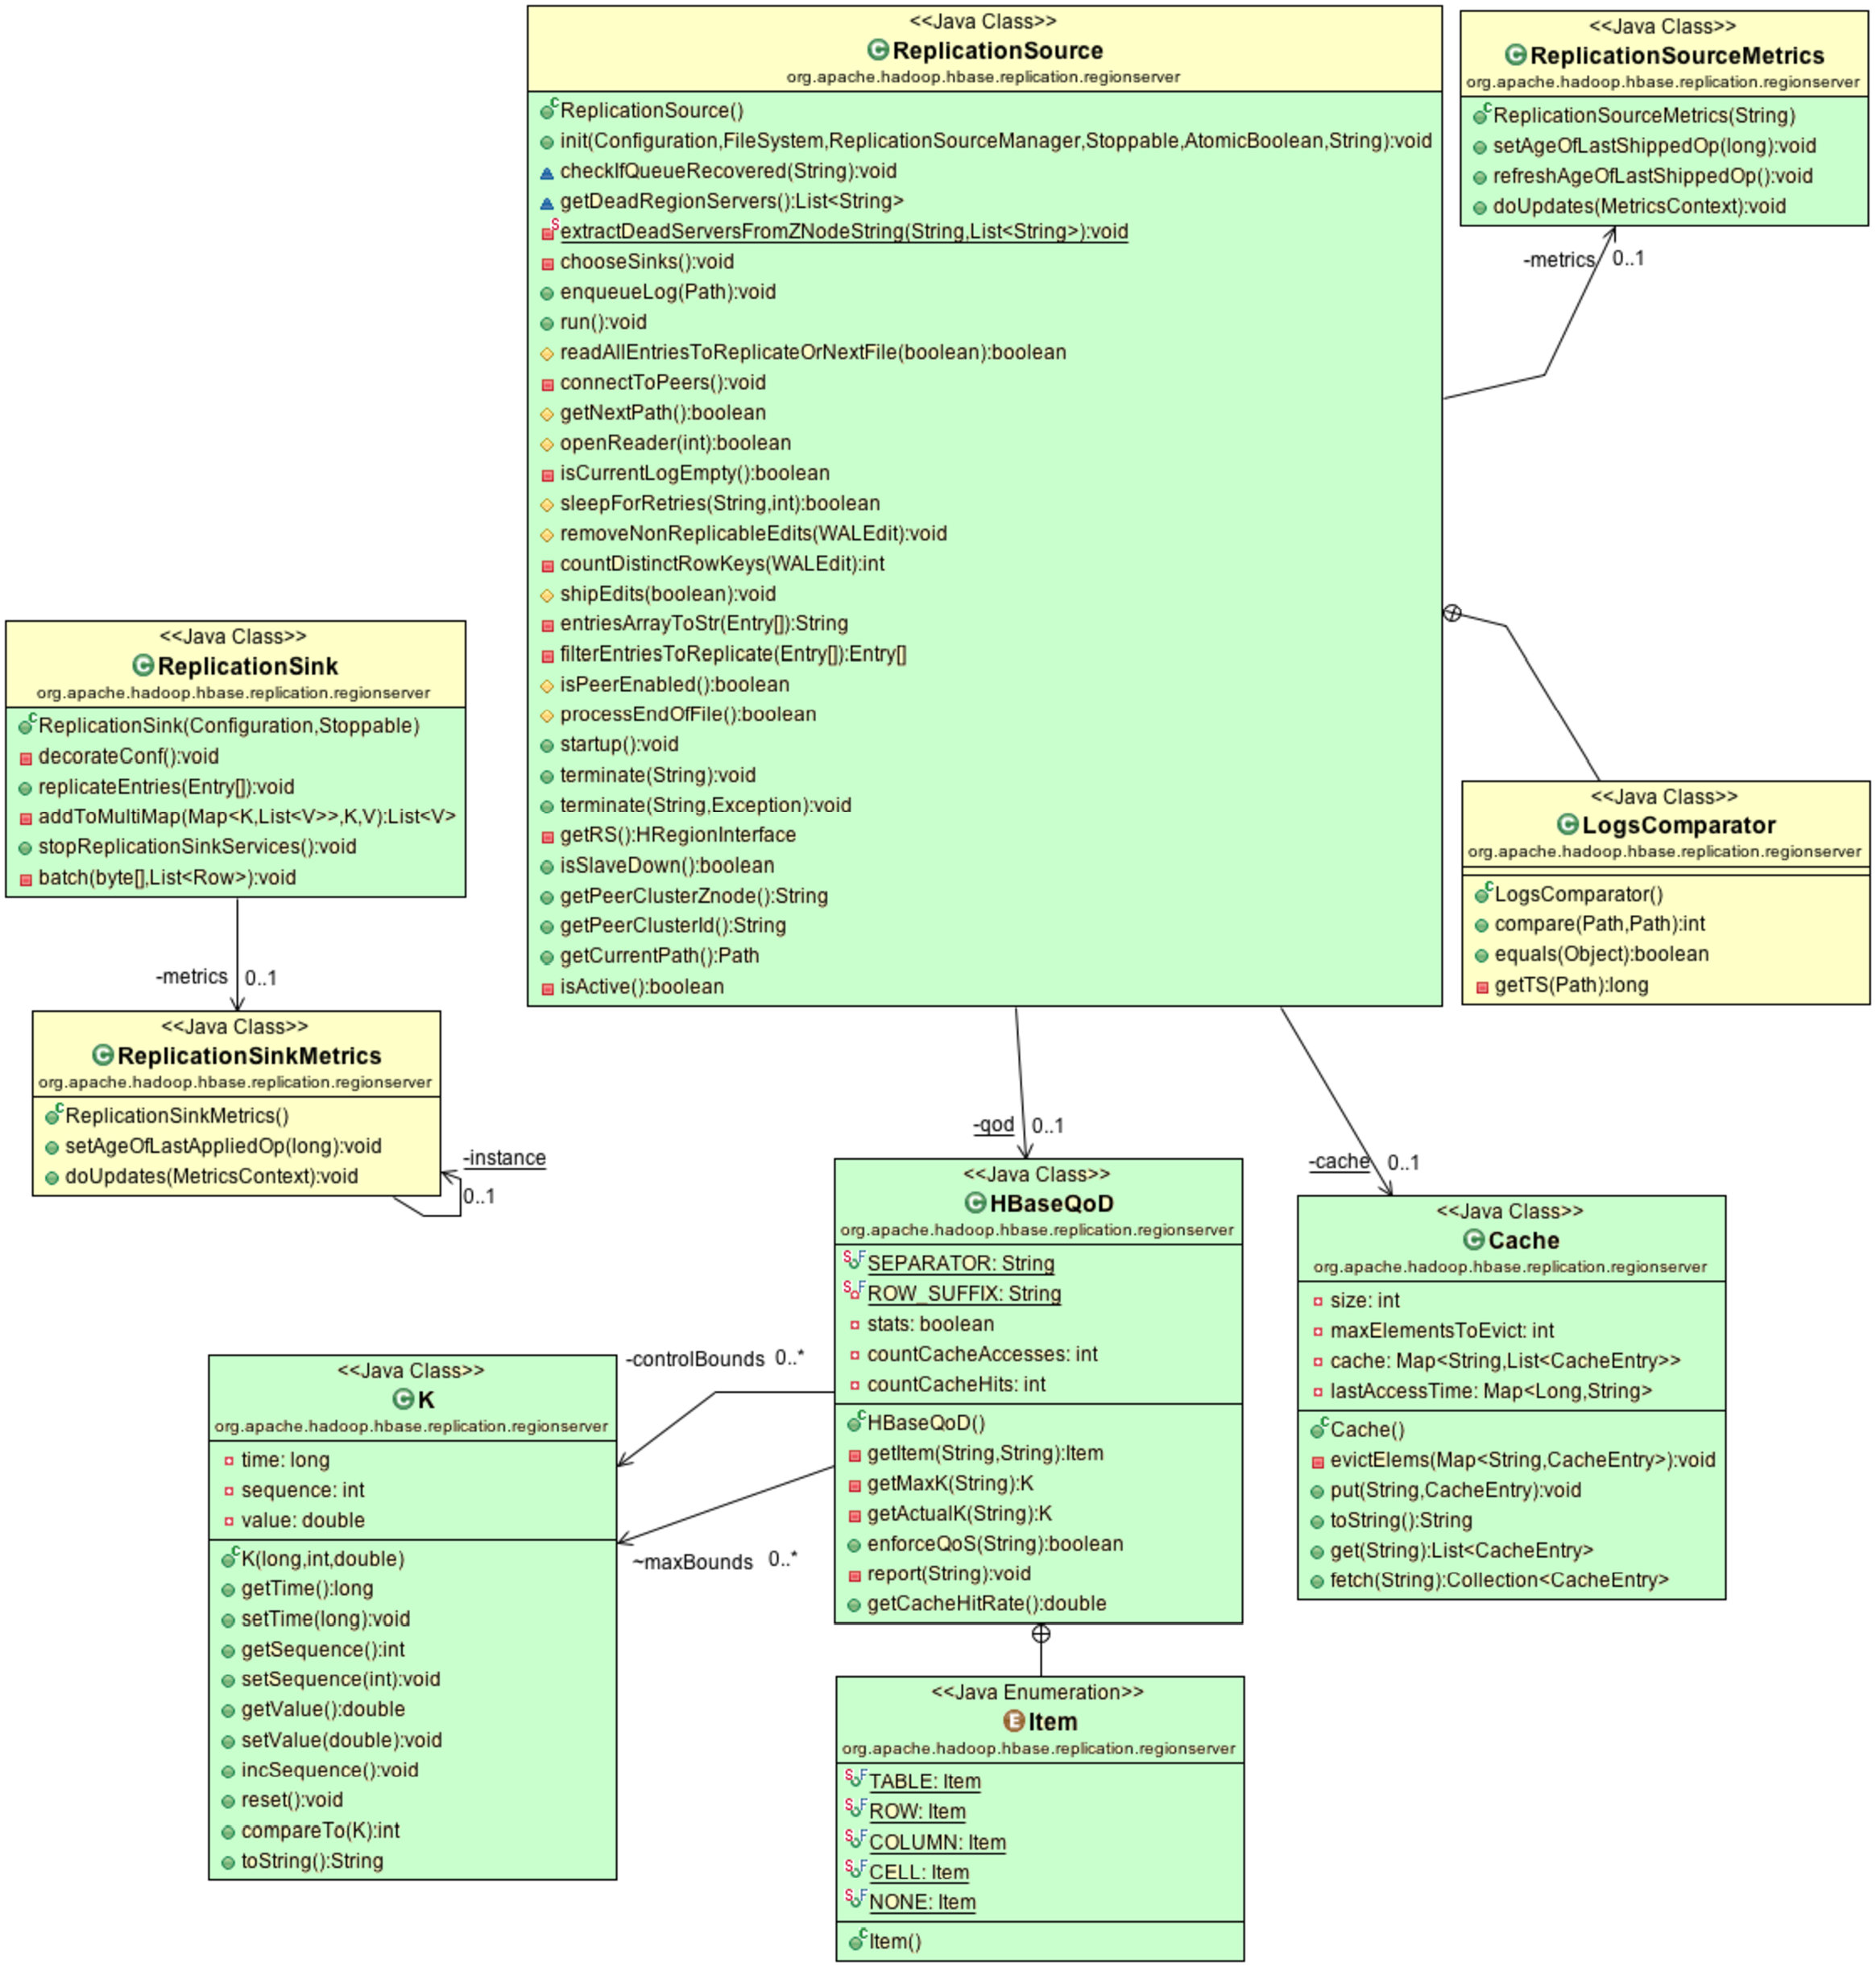
\includegraphics[width=1.0\linewidth]{figs/HBaseQoD-class-diagram.pdf}
\caption{HBase-QoD class diagram}
\label{fig-class-diagram}
\end{figure}



\section{Software Architecture}
%Class Diagram of relevant classes of each HBase instance and your new classes, and classes that have been modified in their interface/methods/public properties.
In the following Figure~\ref{fig-class-diagram} it is depicted the main class diagrams for the architecture solution. Highlighted diagrams in \emph{green} are classes we have introduced into the system or modified in the case of partially highlighted. The main components are the HBaseQoD and the function \emph{filterEntriesToReplicate} where resides the main Algorithm~\ref{algo1} for the consistency enforcement of data semantics we see in \ref{architecture:consistency}.


%this may fall into chapter 4, and is a way of making the bridge to the real implementation details in Chap.4.
Regarding operation grouping, the same logic applies to batches of operations which are grouped based on data dependencies or container-id most restrictive vector field (e.g sequence).


\subsection*{Summary}
This Chapter described the core aspects of our HBase-QoD proposal, addressing its architecture, regarding system, network and software components. We also described the relevant aspects that make consistency enforcement more flexible and aware of user/developer semantics, driven by QoD consistency vectors, followed by the operation/update grouping semantics also provided.

%This is the main outline of the architecture of the system. Next chapter digs into the details of the solution and its technical implementation. 